\chapter{Formato Open CVN, validación y herramienta de gestión}
\label{cap:formato_herramienta}

El Capítulo~\ref{cap:pipeline} describió cómo el pipeline transforma el
paquete oficial CVN en un modelo conceptual y en un artefacto JSON Schema
trazable. El presente capítulo presenta el resultado funcional de ese
trabajo: el formato Open CVN JSON que consumen las aplicaciones, el parser y
el validador públicos que lo comprueban, los mecanismos de importación desde
currículos ya existentes, y la herramienta local que demuestra el uso
completo del sistema. Ninguno de estos elementos desplaza la aportación
principal del trabajo, ya presentada en los capítulos anteriores: son su
consecuencia operativa, no un objetivo en sí mismos.

\section{El formato Open CVN JSON}
\label{sec:formato_json}

Todo documento Open CVN es un objeto JSON con cuatro campos en su raíz:

\begin{itemize}
  \item \texttt{schema\_version}: identifica la versión del formato, no la
  del JSON Schema.

  \item \texttt{metadata}: describe el documento, no su contenido
  curricular.

  \item \texttt{curriculum}: contiene la información curricular propiamente
  dicha.

  \item \texttt{extensions}: opcional, reservado para metadatos específicos
  de una herramienta o proyecto concreto.
\end{itemize}

El campo \texttt{curriculum} organiza la información por área conceptual del
dominio, en lugar de por estructura XML o por módulo generado: \texttt{identity}
describe a la persona titular y es un único objeto, mientras que
\texttt{education}, \texttt{research}, \texttt{professional\_experience},
\texttt{achievements} y \texttt{other} son listas de entradas repetidas. Cada
entrada de una lista declara un \texttt{id} local opcional, un \texttt{type}
conceptual estable, un objeto \texttt{data} con los campos propios de la
entrada y, opcionalmente, un bloque \texttt{trace} con los códigos CVN y las
rutas XML de los que procede.

Los campos que remiten a una tabla de valores controlados, ya introducidos en
la Sección~\ref{sec:pipeline_politica_semantica}, comparten una misma forma
en el JSON: un objeto con \texttt{code}, \texttt{label}, \texttt{source} y,
cuando procede, \texttt{raw\_value} o \texttt{uri}. El campo de sexo del
ejemplo utilizado en el capítulo anterior se representa, siguiendo esta
forma, como \texttt{\{"code": "000", "label": "Mujer", "source":
"CVN\_SEX\_A"\}}. Esta misma forma se reutiliza tanto para las enumeraciones
cerradas como para los catálogos abiertos: lo único que cambia entre ambos
casos es si el validador puede restringir \texttt{code} a un conjunto
cerrado de valores o debe aceptar cualquier valor declarado. El
Código~\ref{cod:formato_raiz} recoge esta estructura raíz en su forma
mínima, sin ningún dato curricular.

\begin{code}[htbp]
\begin{lstlisting}[language=, basicstyle=\small\ttfamily, breaklines=true]
{
  "schema_version": "0.1.0",
  "metadata": {
    "language": "es",
    "policy": {"name": "default_cvn_semantic_policy", "version": "0.1.0"}
  },
  "curriculum": {
    "identity": {},
    "education": [],
    "research": [],
    "professional_experience": [],
    "achievements": [],
    "other": []
  }
}
\end{lstlisting}
\caption{Estructura raíz mínima de un documento Open CVN JSON.}
\label{cod:formato_raiz}
\end{code}

\section{Parser y validador}
\label{sec:formato_parser}

El sistema expone un contrato público de análisis y validación con cuatro
funciones: una para leer Open CVN JSON, otra para validarlo explícitamente,
y dos más para importar currículos existentes en CVN XML y en CVN PDF. Las
cuatro funciones devuelven una misma estructura de resultado, con un estado
de validación entre cinco valores posibles: sin ejecutar, válido, válido con
avisos, inválido o fallido; una lista de errores y otra de avisos, cada uno
con un código estable; y una traza que conserva el formato de origen, los
códigos CVN detectados y las rutas XML asociadas.

Un documento se acepta con avisos, en lugar de aceptarse sin más, cuando
supera la validación estructural y en tiempo de ejecución pero presenta
indicios semánticos conservadores: por ejemplo, una entrada cuyo tipo
conceptual no coincide con la sección en la que aparece, o una referencia
controlada sin ningún campo de \texttt{code}, \texttt{label}, \texttt{raw\_value}
ni \texttt{uri}. Estos avisos nunca convierten un documento válido en
inválido; se limitan a señalar un caso semánticamente atípico para que
pueda revisarse.

La Figura~\ref{fig:formato_flujo_validacion} recorre el flujo completo desde
la entrada, en cualquiera de los tres formatos admitidos, hasta la
clasificación final del resultado.

\begin{figure}[htbp]
  \centering
  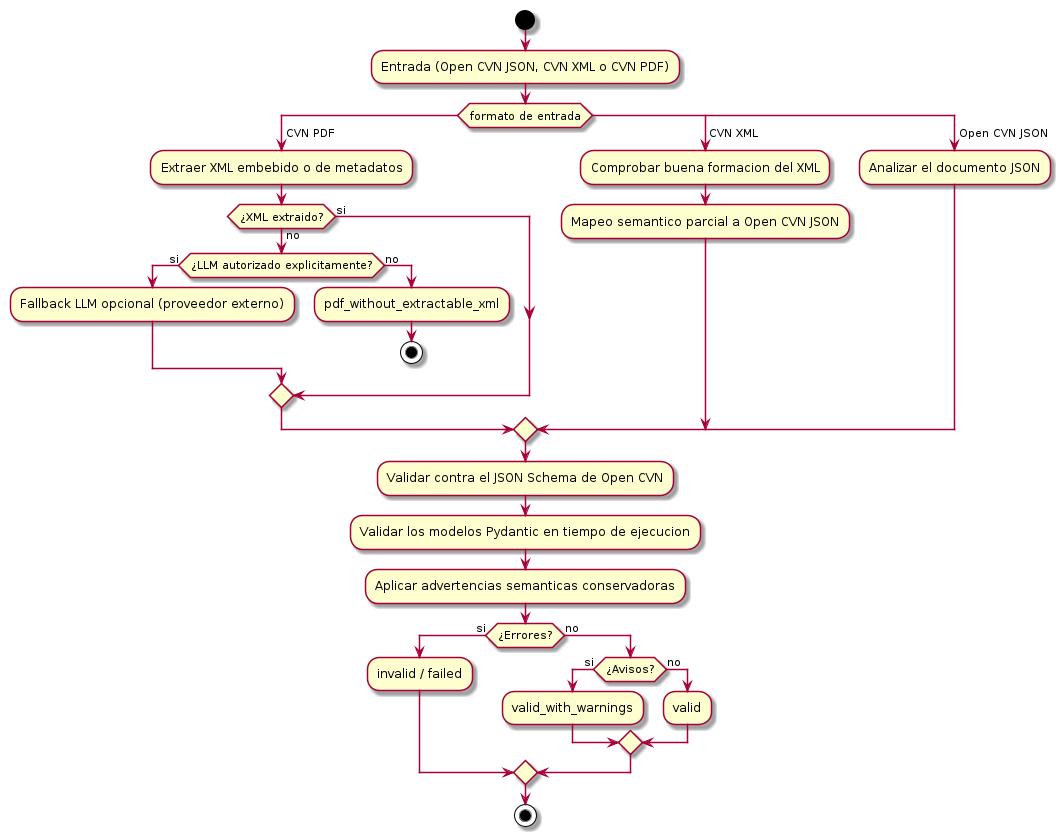
\includegraphics[width=0.85\textwidth]{figs/open_cvn_import_validation_flow.png}
  \caption{Flujo de importación y validación de currículos hacia Open CVN.}
  \label{fig:formato_flujo_validacion}
\end{figure}

\section{Importación de currículos existentes}
\label{sec:formato_importacion}

La importación de Open CVN JSON ya validado es el caso directo: el documento
se analiza y se valida contra el JSON Schema y contra los modelos de dominio,
sin ninguna transformación adicional.

La importación desde CVN XML es semántica parcial: el documento se comprueba
como XML bien formado y, a continuación, los elementos y campos reconocidos
se traducen a secciones de Open CVN utilizando las mismas anotaciones de
trazabilidad del JSON Schema descritas en el
Capítulo~\ref{cap:pipeline}. Los elementos no reconocidos no se descartan en
silencio: quedan preservados en diagnósticos de importación y, cuando
procede, en la sección \texttt{other} del currículo resultante. Esta
importación no debe interpretarse como un conversor completo de cualquier
CVN XML real, sino como un mapeo creciente sobre los casos ya cubiertos.

La importación desde CVN PDF prioriza siempre la vía determinista: si el PDF
conserva el XML CVN embebido, o XML en sus metadatos, ese XML se extrae y
sigue el mismo camino que la importación XML. Solo cuando esa extracción
determinista no es posible, y únicamente si la persona usuaria lo autoriza de
forma explícita, se recurre a un proveedor de modelos de lenguaje (LLM) como
alternativa opcional. El resultado del proveedor externo se almacena
únicamente después de validarse como Open CVN JSON, y queda marcado en las
extensiones del documento como asistido por LLM, de modo que nunca se
presenta como equivalente a una importación determinista.

\section{Herramienta local de gestión}
\label{sec:formato_herramienta_local}

La herramienta local demuestra el uso completo del formato y de los
mecanismos anteriores mediante una interfaz de línea de órdenes. Su modelo de
datos distingue un currículo maestro, que representa la versión completa de
referencia, de versiones derivadas que seleccionan secciones o entradas
concretas de ese maestro para un propósito determinado, como una
convocatoria o una solicitud específica. Toda la información se almacena en
un fichero SQLite local de un único usuario.

El Código~\ref{cod:formato_maestro} y el Código~\ref{cod:formato_derivada}
muestran, de forma reducida, un currículo maestro con una entrada de
investigación y la versión derivada que excluye dicha entrada, tal y como
quedaría tras ejecutar \texttt{versions exclude} sobre el maestro: el resto
del currículo permanece intacto, y la versión derivada registra en sus
extensiones qué selección se aplicó, lo que permite regenerarla de forma
determinista a partir del maestro en lugar de mantenerla como una copia
independiente que pueda divergir silenciosamente de su origen. La
Tabla~\ref{tab:formato_comandos} resume, además, los comandos principales de
la herramienta.

\begin{table}[htbp]
  \centering
  \footnotesize
  \renewcommand{\arraystretch}{1.45}
  \caption{Comandos principales de la herramienta local de gestión.}
  \label{tab:formato_comandos}
  \begin{tabular}{p{0.28\textwidth} p{0.58\textwidth}}
    \hline
    \textbf{Comando} & \textbf{Función} \\
    \hline
    \texttt{store init} & Inicializa el almacenamiento SQLite local \\
    \texttt{json import} & Importa un documento Open CVN JSON, opcionalmente como maestro \\
    \texttt{pdf import} & Importa un CVN PDF, con extracción determinista y LLM opcional \\
    \texttt{versions derive} & Crea una versión derivada a partir del maestro \\
    \texttt{versions list} & Lista las versiones almacenadas \\
    \texttt{versions sections} / \texttt{entries} & Explora las secciones y entradas de una versión \\
    \texttt{versions include} / \texttt{exclude} & Selecciona o excluye una sección o entrada de una versión derivada \\
    \texttt{versions metadata} & Asigna metadatos descriptivos a una versión derivada \\
    \texttt{json export} & Exporta una versión almacenada como Open CVN JSON \\
    \texttt{latex export} & Exporta una versión almacenada a LaTeX \\
    \texttt{pdf generate} & Compila la exportación LaTeX a PDF cuando hay un motor TeX disponible \\
    \hline
  \end{tabular}
\end{table}

\begin{code}[htbp]
\begin{lstlisting}[language=, basicstyle=\footnotesize\ttfamily, breaklines=true]
{
  "schema_version": "0.1.0",
  "curriculum": {
    "identity": {
      "sex": {
        "code": "000",
        "label": "Mujer",
        "source": "CVN_SEX_A"
      }
    },
    "research": [
      {
        "id": "research-001",
        "type": "research.publication",
        "data": {"title": "Open CVN data representation"}
      }
    ]
  }
}
\end{lstlisting}
\caption{Currículo maestro reducido, con una entrada de investigación.}
\label{cod:formato_maestro}
\end{code}

\begin{code}[htbp]
\begin{lstlisting}[language=, basicstyle=\footnotesize\ttfamily, breaklines=true]
{
  "schema_version": "0.1.0",
  "curriculum": {
    "identity": {
      "sex": {
        "code": "000",
        "label": "Mujer",
        "source": "CVN_SEX_A"
      }
    },
    "research": []
  },
  "extensions": {
    "x-open-cvn.versioning": {
      "version_name": "publica",
      "version_kind": "derived",
      "selection": {
        "mode": "include_all",
        "excluded_pointers": ["/curriculum/research/0"]
      }
    }
  }
}
\end{lstlisting}
\caption{Versión derivada ``publica'' del mismo currículo, con la entrada de investigación excluida.}
\label{cod:formato_derivada}
\end{code}

\section{Alcance funcional y garantías}
\label{sec:formato_alcance}

No todos los flujos descritos en este capítulo ofrecen el mismo nivel de
garantía, y conviene distinguirlos con precisión antes de la evaluación del
sistema en el Capítulo~\ref{cap:evaluacion}. Los cuatro flujos principales se sitúan en puntos
distintos entre una garantía determinista y una aproximación parcial y
documentada:

\begin{itemize}
  \item \textbf{Validación de Open CVN JSON.} La validación estructural
  contra el JSON Schema y la validación en tiempo de ejecución contra los
  modelos Pydantic son deterministas y reproducibles para cualquier
  documento Open CVN JSON: dado el mismo documento, el resultado de la
  validación es siempre el mismo, y no depende de heurísticas ni de
  servicios externos.

  \item \textbf{Importación desde CVN XML.} Es un mapeo semántico parcial,
  creciente sobre los casos ya cubiertos por el sistema. No debe
  presentarse ni interpretarse como una conversión completa de cualquier CVN
  XML real: los elementos no reconocidos se preservan como diagnóstico, pero
  no se traducen automáticamente al modelo Open CVN.

  \item \textbf{Importación asistida por LLM.} Es opcional y depende del
  proveedor externo configurado en cada caso. Su resultado nunca se acepta
  directamente: debe pasar primero por la misma validación de Open CVN JSON
  que cualquier otro documento, exactamente igual que los dos flujos
  anteriores.

  \item \textbf{Generación de PDF.} Depende de que exista un motor LaTeX
  disponible en el entorno de ejecución. Su ausencia no es un fallo del
  sistema ni impide el resto de los flujos: la importación, la validación,
  el almacenamiento y la exportación a JSON o LaTeX siguen funcionando sin
  necesidad de generar PDF.
\end{itemize}

El Capítulo~\ref{cap:evaluacion} retoma estas cuatro distinciones para evaluar de forma
sistemática qué partes del sistema ofrecen garantías fuertes y cuáles deben
entenderse como una aproximación parcial y documentada.
